%\UseRawInputEncoding
\documentclass{article}
\setcounter{secnumdepth}{0}
\usepackage[T1]{fontenc}
\usepackage[utf8]{inputenc}
%\usepackage[latin1]{inputenc}
%\usepackage[english, norsk]{babel}
\usepackage{filecontents}
\usepackage{tcolorbox}
\usepackage{url}
\usepackage{etoolbox}
\usepackage{framed}
\usepackage{framed, color}
\usepackage{xcolor}
\usepackage{mdframed}
\usepackage{float}
\usepackage{gensymb}
\usepackage{amsmath}
\usepackage{amsfonts}

\definecolor{Black}{rgb}{0.0, 0.0, 0.0}

%Definer kode
\usepackage{listings}
\usepackage{color}
\definecolor{dkgreen}{rgb}{0,0.6,0}
\definecolor{gray}{rgb}{0.5,0.5,0.5}
\definecolor{mauve}{rgb}{0.58,0,0.82}

\lstset{frame=tb,
extendedchars = true,
texcl=true,
  language=C++,
  aboveskip=3mm,
  belowskip=3mm,
  showstringspaces=false,
  columns=flexible,
  basicstyle={\small\ttfamily},
  numbers=none,
  numberstyle=\tiny\color{gray},
  keywordstyle=\color{blue},
  commentstyle=\color{dkgreen},
  stringstyle=\color{mauve},
  breaklines=true,
  breakatwhitespace=true,
  tabsize=3
}

\usepackage[colorlinks]{hyperref}
\hypersetup{citecolor=Black}
\hypersetup{linkcolor=Black}
\hypersetup{urlcolor=Black}
\usepackage{cleveref}


\setlength{\parindent}{0em}
\setlength{\parskip}{1em}
%\renewcommand{\baselinestretch}{2.0}

%\renewcommand\thesubsection{\alph{subsection}}

\renewcommand{\figurename}{Figure}
\begin{document}
\author{Kent Odde}
\title{Title}

\maketitle
\thispagestyle{empty}
\begin{center}
\includegraphics[width=\linewidth,height=0.2\textheight,keepaspectratio]{img/USN.png}
\end{center}
\newpage

\tableofcontents

\newpage

\section{Abstract}
This is my submission for the home exam in Discrete Mathmatics, fall 2020. 



%Innholdsfortegnelse
\section{Introduction}
The assignment consists of implementing the ElGamal encryption algorithm, in a programming language of my own choosing. As a requirement for the implementation is speed, I found the most suitable language for the task to be C++. Luckily this is also the language I'm most proficient in. 

One downsize of using C++ is the fact that there exists no built in support for large numbers. Building my own library for this would be to time-consuming, so I decided to make use of the Gnu Multiple Precision library (GMP)\cite{GMP}.

Quite a bit of overhead were required to encrypt larger inputs. However, because this course is concerned with the mathematics behind ElGamal and the fact that the professor wanted a short paper, I will not cover this part of the implementation to a detailed extent. 


\subsection{ElGamal}
ElGamal is an asymmetric encryption scheme based on Diffie-Hellman. That it is asymmetric means that the algorithm uses two different keys for encryption and decryption. As encouraged by the professor, I have used the Wikipedia article\cite{WIKI} as my main source of information on ElGamal. Instead of reiterating the details of the algorithm from the article, I will just focus on the main points here. 

We choose a cyclic group G, with a generator g. The private key is denoted by \textit{x}. We use the private key to generate a part of the public key, \textit{h}:

\begin{equation}
h := g^{x}
\end{equation}

If we choose a bad g, the discrete logarithm problem which gives ElGamal its security, will decrease in complexity. 

\section{Implementation}


\subsection{Overhead}

\subsubsection{Padding}
Asymmetric encryption algorithms like RSA and ElGamal, requires a padding scheme in order to make the length of all strings uniform and henceforth increase the security. A common padding scheme for RSA is PKCS\#1.5. As it was hard to find sources for padding schemes commonly used with ElGamal, my choice also fell on PKCS for this implementation. 

A visualization of the scheme can be seen in figure \ref{rPKCS}.  


\begin{figure}[H]
 \centering
  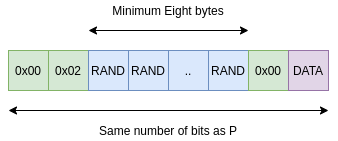
\includegraphics[width=300pt]{img/padding.png}
 \caption{PKCS padding scheme}
 \label{rPKCS}
 \end{figure}

\subsubsection{Block Handling}

ElGamal is not a common choice for encrypting larger texts, however after conversations with the lecturer, I understood that this was a requirement for this assignment. To keep the overhead to a minimum, ECB(Electronic Codebook) was chosen. An illustration of ECB can be seen in figure \ref{rECB}. If the plaintext is larger than the number of bits of P, we divide it up into blocks, encrypt them seperately, and concatenate them. 
%DETTE BILDET MÅ BYTTES UT, VISER DEC OG IKKE ENC!!!!!!!!!!!!!!!!!!!!!!!!!!!!!!!!!!!!!!!!!!!
\begin{figure}[H]
 \centering
  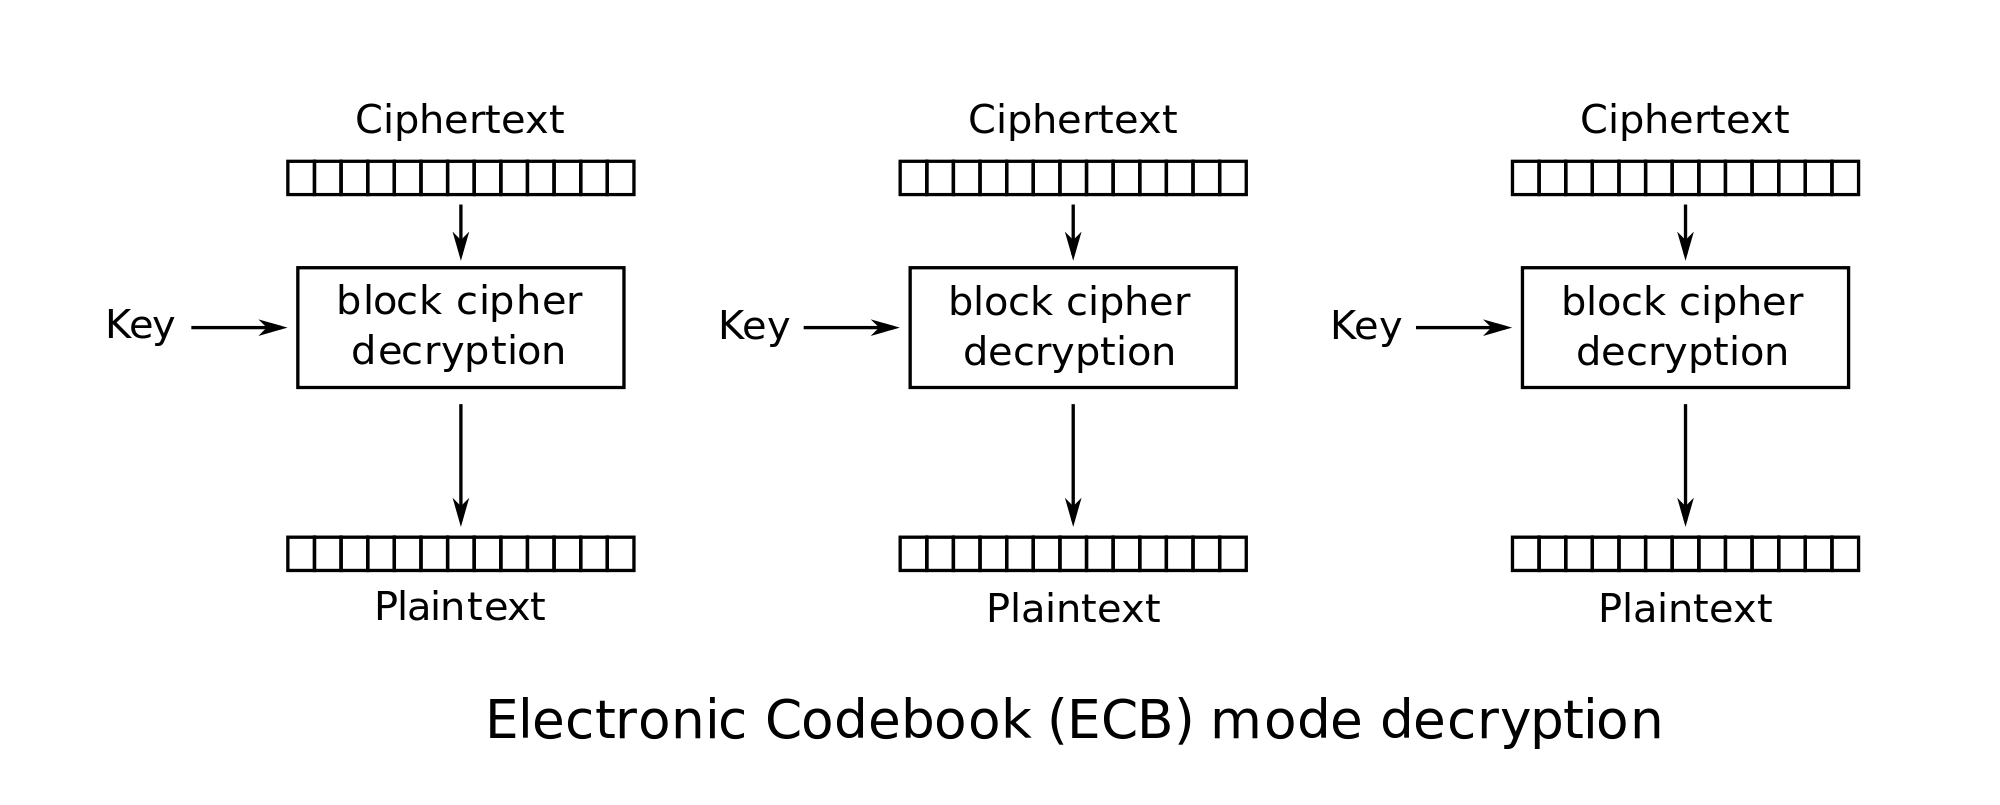
\includegraphics[width=300pt]{img/ECB.png}
 \caption{Electronic Codebook\cite{ECB}}
 \label{rECB}
 \end{figure}

An extra complication with ElGamal is that the algorithm produces two numbers, in which the size of bits may vary. In order to be able to parse the concatenated strings later, I decided to prepend zeroes to c1 and c2, until their length were at 512 bits.

Putting the padding together with Elgamal and and the post-encryption padding the full overview of this implementation encrypts a string, can be seen in figure \ref{rOVERHEAD}

\begin{figure}[H]
 \centering
  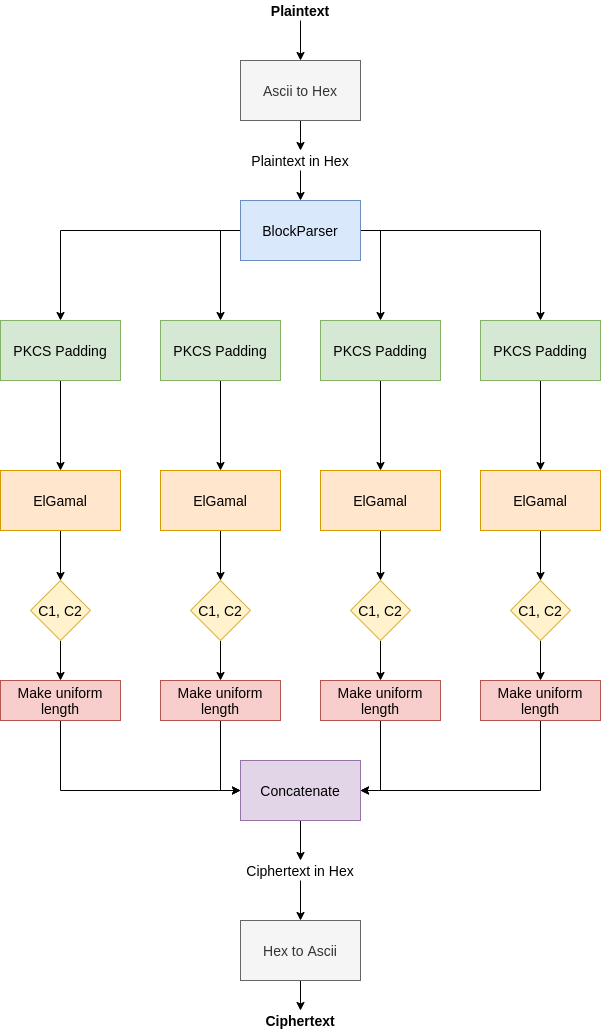
\includegraphics[width=300pt]{img/overview.png}
 \caption{Overview of the overhead}
 \label{rOVERHEAD}
 \end{figure}


\subsection{ElGamal}

\subsubsection{Generating Keys}
\begin{equation}
G = (\mathbb{Z}/p)^{*}
\end{equation}

\begin{equation}
q = ord(G) = ord(\mathbb{Z}/p)^{*} = p-1
\end{equation}

\begin{equation}
privateKey = x \in \{1, ..., q-1\}
\end{equation}

\begin{equation}
h := g^{x}
\end{equation}

\begin{equation}
publicKey  = (G, q, g, h)
\end{equation}

\textbf{Finding and choosing a generator}

\begin{equation}
Y = g^{x} \bmod p
\end{equation}

	For every value of x, we should get a unique value of Y

	All generators are factors of p-1




\subsubsection{Encryption}

We choose a random number y, from the set
\begin{equation}
\{1, ..., q-1\}
\end{equation}


\subsubsection{Decryption}



%Konklusjon
\section{Conclusion}






%Vedlegg
\section{Appendices}


\newpage
%Referanse
%\section{Referanser}

\nocite{*}
\bibliographystyle{plain}
\bibliography{ref}

\addcontentsline{toc}{section}{References}

\end{document}
